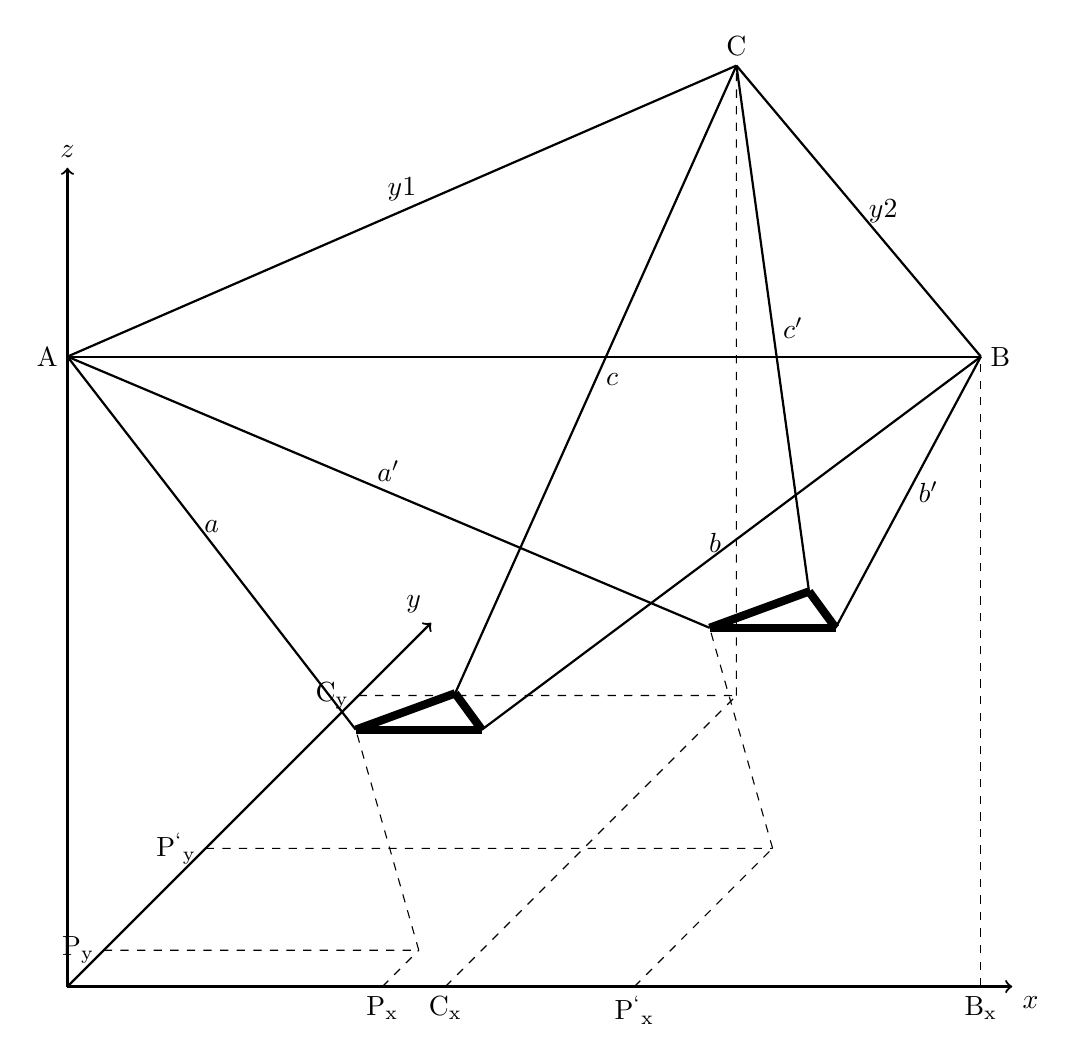
\begin{tikzpicture}[scale=0.8]		   
	\coordinate 	[label=left:	A](A) 	at 	(0,10,0);
	\coordinate 	[label=right:	B](B) 	at 	(14.5,10,0);
	\coordinate 	[label=above:	C](C) 	at 	(6,10,-12);
	\coordinate(P1) 	at 	(4,3.5,-1.5);
	\coordinate(P1') 	at 	(8,3.5,-5.7);
	\coordinate(P2) 	at 	(6,3.5,-1.5);
	\coordinate(P2') 	at 	(10,3.5,-5.7);
	\coordinate(P3) 	at 	(5,3.5,-3);
	\coordinate(P3') 	at 	(9,3.5,-7.2);
	\coordinate		[label=left:	P\textsubscript{y}](YP)	at 	(0,0,-1.5);
	\coordinate		[label=below:	P\textsubscript{x}](XP)	at 	(5,0,0);
	\coordinate		[label=left:	P\textsuperscript{`}\textsubscript{y}](YP')	at 	(0,0,-5.7);
	\coordinate		[label=below:	P\textsuperscript{`}\textsubscript{x}](XP')	at 	(9,0,0);
	\coordinate		[label=below:	B\textsubscript{x}]				(XB)	at 	(14.5,0,0);
	\coordinate		[label=below:	C\textsubscript{x}](XC)	at 	(6,0,0);
	\coordinate		[label=left:	C\textsubscript{y}](YC)	at 	(0,0,-12);

	\draw[thick,->] (0,0,0) 		-- 	(15,0,0) 	node[anchor=north west]	{$x$};
	\draw[thick,->] (0,0,0) 		-- 	(0,0,-15)	node[anchor=south east]	{$y$};
	\draw[thick,->] (0,0,0) 		-- 	(0,13,0) 	node[anchor=south]		{$z$};	
	\draw[thick] 	(A) 			-- 	(B) 		;		
	\draw[thick] 	(B) 			-- 	(C) 		node[midway,right]		{$y2$};	
	\draw[thick] 	(C) 			-- 	(A) 		node[midway,above]		{$y1$};	
	\draw[thick] 	(A) 			-- 	(P1) 		node[midway,above]		{$a$};
	\draw[thick] 	(A) 			-- 	(P1') 		node[midway,above]		{$a'$};
	\draw[thick] 	(B) 			-- 	(P2) 		node[midway,left]		{$b$};
	\draw[thick] 	(B) 			-- 	(P2') 		node[midway,right]		{$b'$};
	\draw[thick] 	(C) 			-- 	(P3) 		node[midway,right]		{$c$};
	\draw[thick] 	(C) 			-- 	(P3') 		node[midway,right]		{$c'$};
	\draw[line width =3pt] 	(P1) 			-- 	(P2) 		;
	\draw[line width =3pt] 	(P2) 			-- 	(P3) 		;
	\draw[line width =3pt] 	(P3) 			-- 	(P1) 		;
	\draw[line width =3pt] 	(P1') 			-- 	(P2') 		;
	\draw[line width =3pt] 	(P2') 			-- 	(P3') 		;
	\draw[line width =3pt] 	(P3') 			-- 	(P1') 		;
	\draw[dashed,-] (XB) 			-- 	(B) 		;
	\draw[dashed,-] (XC) 			-- 	(6,0,-12);
	\draw[dashed,-] (YC) 			-- 	(6,0,-12);
	\draw[dashed,-] (6,0,-12)	-- 	(C) 		;
	\draw[dashed,-] (XP) 			-- 	(5,0,-1.5) 	;
	\draw[dashed,-] (YP) 			-- 	(5,0,-1.5) 	;
	\draw[dashed,-] (5,0,-1.5) 		-- 	(P1)		;
	\draw[dashed,-] (XP') 			-- 	(9,0,-5.7) 	;
	\draw[dashed,-] (YP') 			-- 	(9,0,-5.7) 	;
	\draw[dashed,-] (9,0,-5.7) 		-- 	(P1')		;
\end{tikzpicture}
\caption{Darstellung der Transformation einer Plattform im Dreidimensionalen} 